\chapter{A Stochastic Recurrence with Sum and Max}

\section{Definition}

Consider the recurrence
\begin{equation}
  \label{eq:yield_indicator}
  Y_{n+2} \stackrel{d}{=} I^{(n)}\left(Y_{U_n}^{(1)} + Y_{n+1-U_n}^{(2)} + 1\right) + J^{(n)}\max\left(Y_{U_n}^{(1)}, Y_{n+1-U_n}^{(2)}\right), \quad Y_1 = Y_2 = 0.
\end{equation}

The context leading to analyzing this recurrence is given in Section~\ref{sec:yield_context}. The variables $I$ and $J$ are Bernoulli with expectation $u$ and $v$ respectively, such that $I + J \le 1$. The variable $U_n$ is uniformly distributed on $\{1, \ldots, n\}$. Superscripts are for independent copies. We assume that all collections of copies are independent. We want to analyze the asymptotic of $Y_n$.

\section{Lower Bounds}
Taking the expectation and using $\max(Y_i, Y_{n+1-i}) \ge \dfrac{1}{2}(Y_i + Y_{n+1-i})$, we get a lower bound sequence
\begin{equation}
  \label{eq:lower_bound_average}
  y_{n+2} = u + \dfrac{2u+v}{n}\sum_{i=1}^{n}y_i, \quad y_1=y_2=0.
\end{equation}
In the case $2u+v > 1$ which aligns with real data (Section \ref{sec:yield_context}), we have $y_n \sim C'n^{2u+v-1}$. Hence we want to prove or disprove that in such case, $\EE[Y_n]\sim Cn^\alpha$ for some $\alpha > 2u+v-1$.

Another lower bound is obtained by using
$$\mathbb{E}[\max(Y_i, Y_{n+1-i})] \ge \max(\mathbb{E}[Y_i], \mathbb{E}[Y_{n+1-i}]) = \max(y_i, y_{n+1-i}) = y_{\max(i, n+1-i)}.$$

That gives another (homogenized) lower bound sequence
\begin{equation}
  \label{eq:recurrence-sum-half-sum-corrected}
  x_{n+2} = \dfrac{2u}{n}\sum_{i=1}^{n}x_i + \dfrac{2v}{n}\sum_{i=\lfloor (n+1)/2 \rfloor}^{n}x_{i}, \quad n \ge 2, \quad  x_1=x_2=1.
\end{equation}

It is proved by induction that $y_n \in \Omega(n^\beta)$, where $\beta$ is the unique solution to
$$2(u+v) - v2^{-\beta} = \beta+1.$$

\section{Attempts}
We want to see if there is $\alpha$ and $C > 0$ such that $X_n = \dfrac{Y_n}{Cn^\alpha}$ converges in distribution to a random variable $X$ of mean 1. Substituting in the recurrence, we get the limit distributional equation
\begin{equation}
  \label{eq:yield_limit_distributional_equation}
  X \stackrel{d}{=} I\left(U^\alpha X^{(1)} + (1-U)^\alpha X^{(2)}\right) + J\max\left(U^\alpha X^{(1)}, (1-U)^\alpha X^{(2)}\right),
\end{equation}

where $U$ is uniformly distributed on $(0,1)$. A subproblem is to prove or disprove that \textit{there exists a unique $\alpha$ such that the equation has a solution with mean 1}. Contraction method with Wasserstein or Zolotarev metrics did not work. That may be because we need to exploit more information of $\alpha$ to prove contraction in a more appropriate space.


\section{Context of the Recurrence}
\label{sec:yield_context}

\begin{note}
  This section can be skipped.
\end{note}

Hyperscan is a regex matching engine. It works based on decomposing regexes into smaller literals and FAs. According to real data \cite{snort_rules_2026}, a pattern consists of many literals. This is confirmed by fitting the dataset to a BST-like model \cite{nicaud2010average} using maximum likelihood. Details are as follows.

Let $\A$ be a finite alphabet and $\T$ be the set of all regexes excluding $\epsilon$ over $\A$.

\begin{definition}[BST-like distribution for regexes]
  We define $p:\T \to [0,1]$ as follows.
  \begin{enumerate}
    \item $\sum\limits_{c\in\A}p(c) = 1$,
    \item $p\left(\vcenter{\hbox{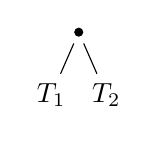
\begin{tikzpicture}[level distance=8mm, sibling distance=7mm, edge from parent/.style={draw, shorten <=1mm}]
                  \node[circle, draw, fill=black, minimum size=1mm, inner sep=0pt] {}
                  child { node {$T_1$} }
                  child { node {$T_2$} };
                \end{tikzpicture}}}\right) = \dfrac{u}{n-2} p(T_1)p(T_2)$, where $|T_1| + |T_2| = n-1$.
    \item $p\left(\vcenter{\hbox{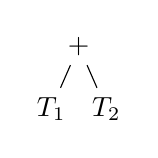
\begin{tikzpicture}[level distance=8mm, sibling distance=7mm]
                  \node{$+$}
                  child { node {$T_1$} }
                  child { node {$T_2$} };
                \end{tikzpicture}}}\right) = \dfrac{v}{n-2} p(T_1)p(T_2)$, where $|T_1| + |T_2| = n-1$.
    \item $p\left(\vcenter{\hbox{\begin{tikzpicture}[level distance=8mm, sibling distance=7mm]
                  \node{$*$}
                  child { node {$T$} };
                \end{tikzpicture}}}\right) = (1-u-v) p(T)$.
  \end{enumerate}
\end{definition}

We want to compute the expected size of the largest all-concatenation component in a regex over all of equivalent forms of its parse tree. The reason is as follows. Take the regex
$$(abc + d)(xy+z) = abcxy + abcxz + dxy + dz.$$
We expect the largest concatenation-component to be in $abcxy$ instead of $abc$ because the former is extracted by Hyperscan. Therefore, a subtree may \textit{yield} its concatenation-component to its parent if the parent is a concatenation node. Recall the construction
$$\T = \sum_{c \in \A} c + \vcenter{\hbox{\begin{tikzpicture}[level distance=8mm, sibling distance=7mm]
        \node{$*$}
        child { node {$\T$} };
      \end{tikzpicture}}} + \vcenter{\hbox{\begin{tikzpicture}[level distance=8mm, sibling distance=7mm, edge from parent/.style={draw, shorten <=1mm}]
        \node[circle, draw, fill=black, minimum size=1mm, inner sep=0pt] {}
        child { node {$\T$} }
        child { node {$\T$} };
      \end{tikzpicture}}} + \vcenter{\hbox{\begin{tikzpicture}[level distance=8mm, sibling distance=7mm]
        \node{$+$}
        child { node {$\T$} }
        child { node {$\T$} };
      \end{tikzpicture}}}.$$
Define the random variables
\begin{enumerate}
  \item $M_n$: the largest concatenation-component that is not inside a Kleene star of a regex of size $n$ \textit{itself},
  \item $Y_n$: the largest concatenation-component that is not inside a Kleene star of a regex of size $n$ that it \textit{yields} to its parent.
\end{enumerate}

We have the following recurrences
\begin{align}
  Y_{n+2}
   & =\begin{cases}
        Y_{U_n}^{(1)} + Y_{n+1-U_n}^{(2)} + 1  & \text{prob. } u,    \\
        \max(Y_{U_n}^{(1)}, Y_{n+1-U_n}^{(2)}) & \text{prob. } v,    \\
        0                                      & \text{prob. } 1-u-v
      \end{cases}                                                                      & Y_1=Y_2=0.                         \label{eq:yield}                           \\
  M_{n+2}
   & = \begin{cases}
         \max(Y_{U_n}^{(1)} + Y_{n+1-U_n}^{(2)} + 1, M_{U_n}^{(1)}, M_{n+1-U_n}^{(2)}) & \text{prob. } u,    \\
         \max(M_{U_n}^{(1)}, M_{n+1-U_n}^{(2)})                                        & \text{prob. } v     \\
         0                                                                             & \text{prob. } 1-u-v
       \end{cases} & M_1=M_2=0.
\end{align}

We have used $Y_n^{(1)}, Y_n^{(2)}, M_n^{(1)}, M_n^{(2)}$ as independent copies of $Y_n$ and $M_n$ respectively, and $U_n$ as a uniform random variable over $\{1, 2, \ldots, n\}$ independent of all $Y_n^{(i)}$ and $M_n^{(i)}$. The recurrence \eqref{eq:yield_indicator} is the distributional version of \eqref{eq:yield}. Note that we can reuse the same $U_n$ and $Y_n^{(i)}$ since the branches to which they are applied cannot be both active.

Due to MLE estimation, it is plausible to assume that $2u+v > 1$ and even $u > v$.